\documentclass{../../assignment}
\usepackage{amsmath}
\usepackage{graphicx}
\usepackage{hyperref}
\usepackage{listings}
\usepackage{float}
\lstset{
numbers=left
}

\coursetitle{Computer Vision II}
\courselabel{CSE 252B}
\exercisesheet{Homework 1}{}
\student{Zhu, Zhongjian}
\university{University of California, San Diego}
\semester{Winter 2017}
\date{\today}

\begin{document}
\begin{problemlist}

\pbitem Line-plane intersection

The line in 3D defined by the join of the points $\mathbf{X_1} = (X_1,Y_1,Z_1,T_1)^ \mathrm{T}$ and $\mathbf{X_2} = (X_2,Y_2,Z_2,T_2)^ \mathrm{T}$ can be represented as a Pl\"ucker matrix L = $\mathbf{X_1X_2^ \mathrm{T} - X_2X_1^ \mathrm{T}}$ or pencil of points $\mathbf{X}(\lambda) = \lambda\mathbf{X_1} + (1 - \lambda)\mathbf{X_2}$. The line intersects the plane $\mathbf{\pi} = (a,b,c,d)^\mathrm{T}$ at the point $\mathbf{X_\mathrm{L}} = \mathrm{L}\pi$ or $\mathbf{X}(\lambda_\pi)$, where $\lambda_\pi$ is determined such that $\mathbf{X}(\lambda_\pi)^\mathrm{T}\pi = 0$. Show that $\mathbf{X}_\mathrm{L}$ is equal to $\mathbf{X}(\lambda_\pi)$ up to scale.
\\
\\
\textbf{Solution}\\
Since $\mathbf{X_\mathrm{L}} = \mathrm{L}\pi$, then
\[ \mathbf{X_\mathrm{L}} = (\mathbf{X_1X_2^ \mathrm{T} - X_2X_1^ \mathrm{T}})\pi =
\begin{bmatrix}
b(X_1Y_2-X_2Y_1)&+&c(X_1Z_2 - X_2Z_1)&+&d(T_2X_1 - T_1X_2)\\
a(X_2Y_1-X_1Y_2)&+&c(T_1Z_2 - Y_2Z_1)&+&d(T_2Y_1 - T_1Y_2)\\
a(X_2Z_1-X_1Z_2)&+&b(Y_2Z_1 - Y_1Z_2)&+&d(T_2Z_1 - T_1Z_2)\\
a(T_1X_2-T_2X_1)&+&b(T_1T_2 - T_2Y_1)&+&c(T_1Z_2 - T_2Z_1)\end{bmatrix}.\]
For $\mathbf{X}(\lambda_\pi)$, from $\mathbf{X}(\lambda_\pi)^\mathrm{T}\pi = 0$, we have
\[ \lambda_\pi = -\frac{aX_2+bY_2+cZ_2+dT_2}{a(X_1-X_2)+b(Y_1-Y2)+c(Z_1-Z_2)+d(T_1-T2)}.\]Let $m = a(X_1-X_2)+b(Y_1-Y2)+c(Z_1-Z_2)+d(T_1-T2)$, then
\[\mathbf{X}(\lambda_\pi) = -\frac{1}{m}
\begin{bmatrix}
b(X_1Y_2-X_2Y_1)&+&c(X_1Z_2 - X_2Z_1)&+&d(T_2X_1 - T_1X_2)\\
a(X_2Y_1-X_1Y_2)&+&c(T_1Z_2 - Y_2Z_1)&+&d(T_2Y_1 - T_1Y_2)\\
a(X_2Z_1-X_1Z_2)&+&b(Y_2Z_1 - Y_1Z_2)&+&d(T_2Z_1 - T_1Z_2)\\
a(T_1X_2-T_2X_1)&+&b(T_1T_2 - T_2Y_1)&+&c(T_1Z_2 - T_2Z_1)\end{bmatrix}.
\]
So, $\mathbf{X}_\mathrm{L} = \mathbf{X}(\lambda_\pi)$.
\\\\
\pbitem Line-quadric intersection

If the pencil of points $\mathbf{X}(\lambda) = \lambda\mathbf{X_1} + (1 - \lambda)\mathbf{X_2}$ represents a line in 3D, the (up to two) real roots of the quadratic polynomial $c_2\lambda_Q^2+c_1\lambda_Q+c_0=0$ are used to solve for the intersection point(s) $\mathbf{X}(\lambda_Q)$. Show that $c_2=\mathbf{X_1}^\mathrm{T}Q\mathbf{X_1}-2\mathbf{X_1}^\mathrm{T}Q\mathbf{X_2}+\mathbf{X_2}^\mathrm{T}Q\mathbf{X_2}$, $c_1=2(\mathbf{X_1}^\mathrm{T}Q\mathbf{X_2}-\mathbf{X_2}^\mathrm{T}Q\mathbf{X_2})$, and $c_0=\mathbf{X_2}^\mathrm{T}Q\mathbf{X_2}$.
\\\\
\textbf{Solution}\\
A 3D point $\mathbf{X}$ is on the quadric $Q$ if and only if $\mathbf{X}^\mathrm{T}Q\mathbf{X}=0$, then
\begin{equation}
(\lambda\mathbf{X_1} + (1 - \lambda)\mathbf{X_2})^\mathrm{T}Q(\lambda\mathbf{X_1} + (1 - \lambda)\mathbf{X_2})=0
\end{equation}
\begin{equation}
\lambda^2\mathbf{X_1}^\mathrm{T}Q\mathbf{X_1}+
\lambda(1-\lambda)\mathbf{X_1}^\mathrm{T}Q\mathbf{X_2}+
\lambda(1-\lambda)\mathbf{X_2}^\mathrm{T}Q\mathbf{X_1}+
(1-\lambda)^2\mathbf{X_2}^\mathrm{T}Q\mathbf{X_2}=0
\end{equation}

Since the transpose of a scalar is itself, from equation(0-1), we have
\begin{equation}
(\mathbf{X_1}^\mathrm{T}Q\mathbf{X_1}-2\mathbf{X_1}^\mathrm{T}Q\mathbf{X_2}+\mathbf{X_2}^\mathrm{T}Q\mathbf{X_2})\lambda^2+
2(\mathbf{X_1}^\mathrm{T}Q\mathbf{X_2}-\mathbf{X_2}^\mathrm{T}Q\mathbf{X_2})\lambda+
\mathbf{X_2}^\mathrm{T}Q\mathbf{X_2}=0
\end{equation}
So, $c_2=\mathbf{X_1}^\mathrm{T}Q\mathbf{X_1}-2\mathbf{X_1}^\mathrm{T}Q\mathbf{X_2}+\mathbf{X_2}^\mathrm{T}Q\mathbf{X_2}$, $c_1=2(\mathbf{X_1}^\mathrm{T}Q\mathbf{X_2}-\mathbf{X_2}^\mathrm{T}Q\mathbf{X_2})$, and $c_0=\mathbf{X_2}^\mathrm{T}Q\mathbf{X_2}$.
\\\\
\pbitem Programming: Automatic feature detection and matching

\begin{figure}[H]
  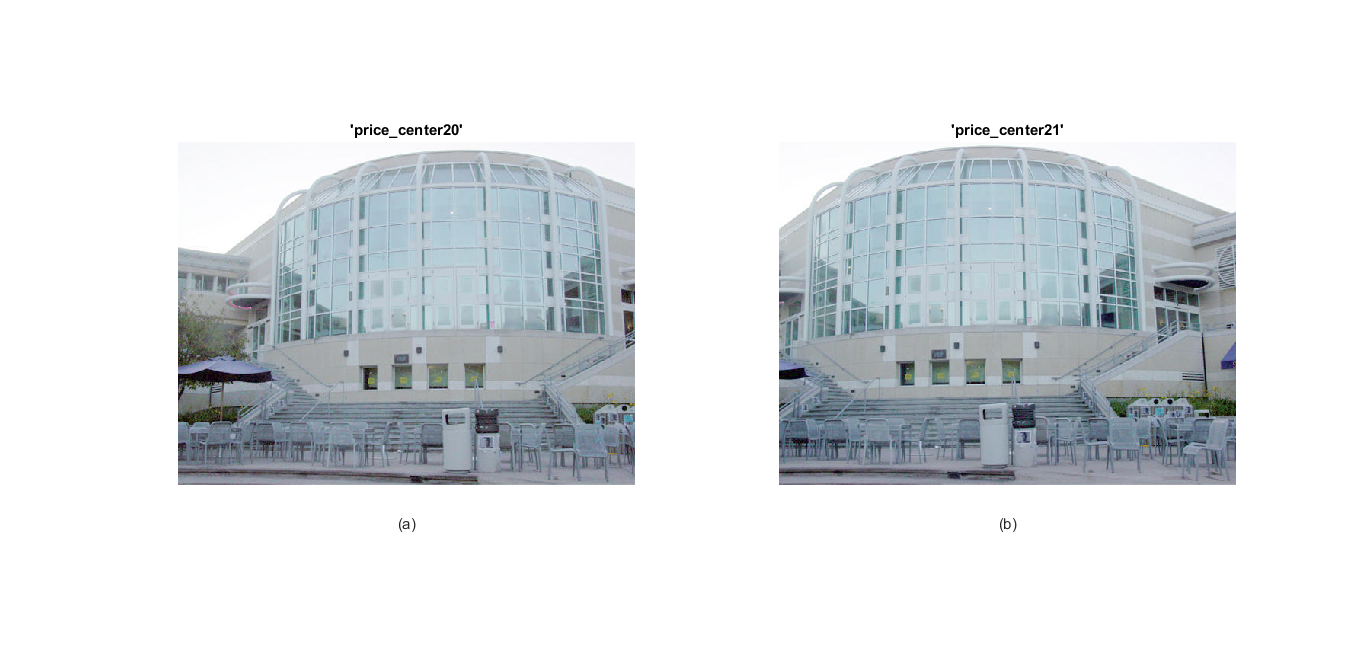
\includegraphics[width=\textwidth]{InputImage}
\caption{(a) shows the image \emph{price\_ center20.JPG}, (b) shows the image \emph{price\_ center21.JPG}.}
% \label{fig:images}
\end{figure}

\begin{enumerate}
\item Feature detection\\
The size of the feature detection window is $11\times11$, 
the minor eigenvalue threshold value is 5, 
the size of the local non-maximum suppression window is $9\times9$.\\
The number of features detected in \emph{price\_ center20.JPG} is 616, and the number of features detected in \emph{price\_ center21.JPG} is 632.

\begin{figure}[H]
  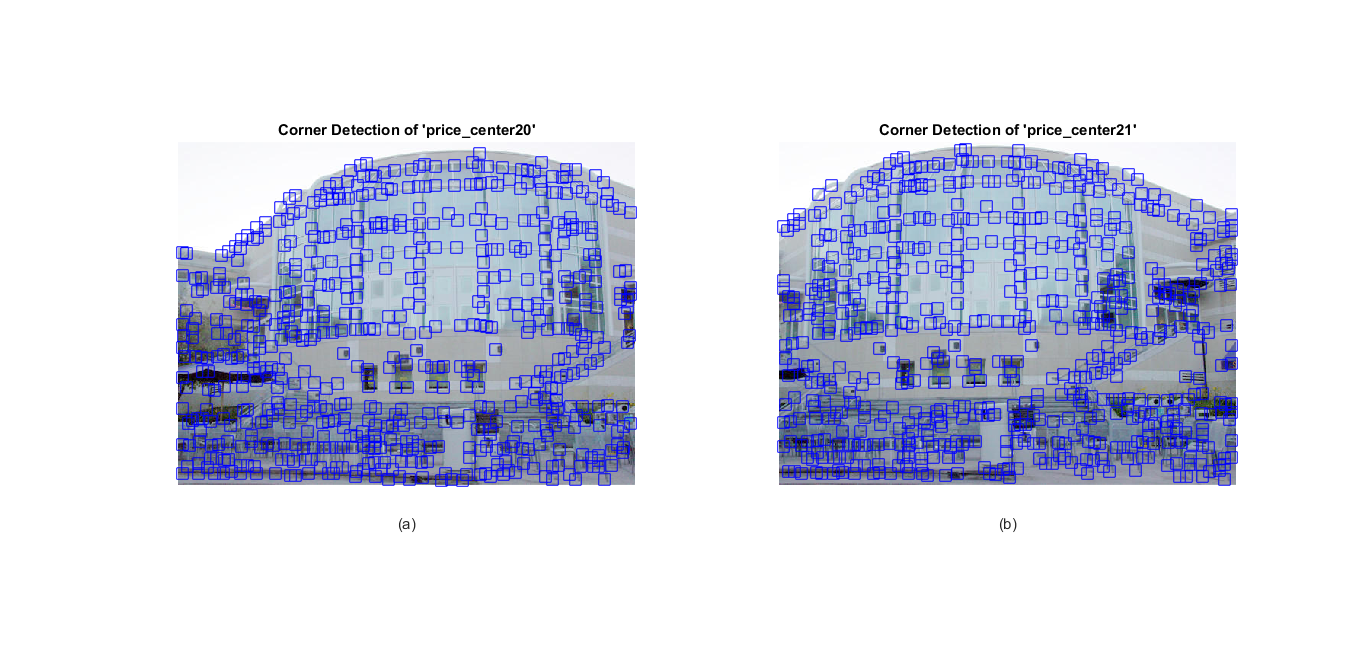
\includegraphics[width=6in]{CornerDetection_NMS}
\caption{(a) shows detected corners(after local nonmaximum suppression) of the image \emph{price\_ center20.JPG}, (b) shows detected corners(after local nonmaximum suppression) of the image \emph{price\_ center21.JPG}.}
% \label{fig:images}
\end{figure}
 
\begin{figure}[H]
  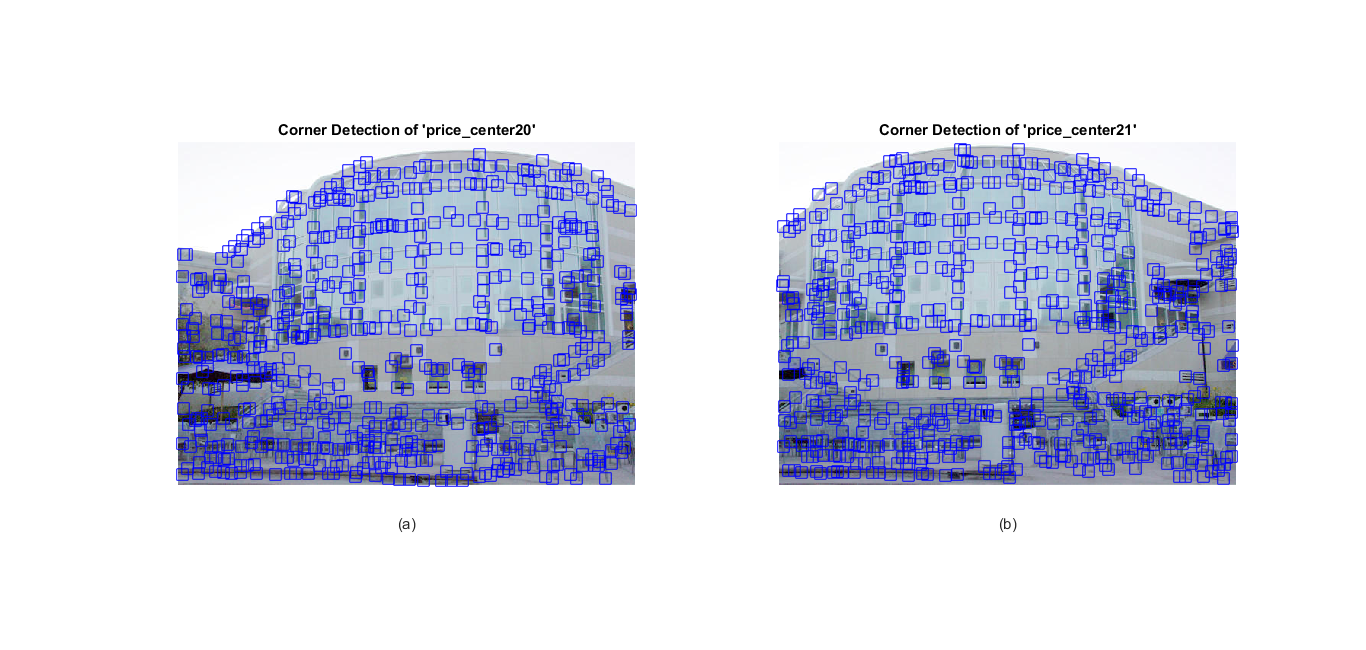
\includegraphics[width=6in]{CornerDetection_Subp}
\caption{(a) shows detected corners(about the subpixel) of the image \emph{price\_ center20.JPG}, (b) shows detected corners(about the subpixel) of the image \emph{price\_ center21.JPG}.}
% \label{fig:images}
\end{figure} 




\item Feature matching\\
The size of the proximity window is $20\times500$, the correlation coefficient threshold value is 0.6, the distance ratio threshold value is 0.9, and the resulting
number of putative feature correspondences is 196.\\
\\
\begin{figure}[H]
  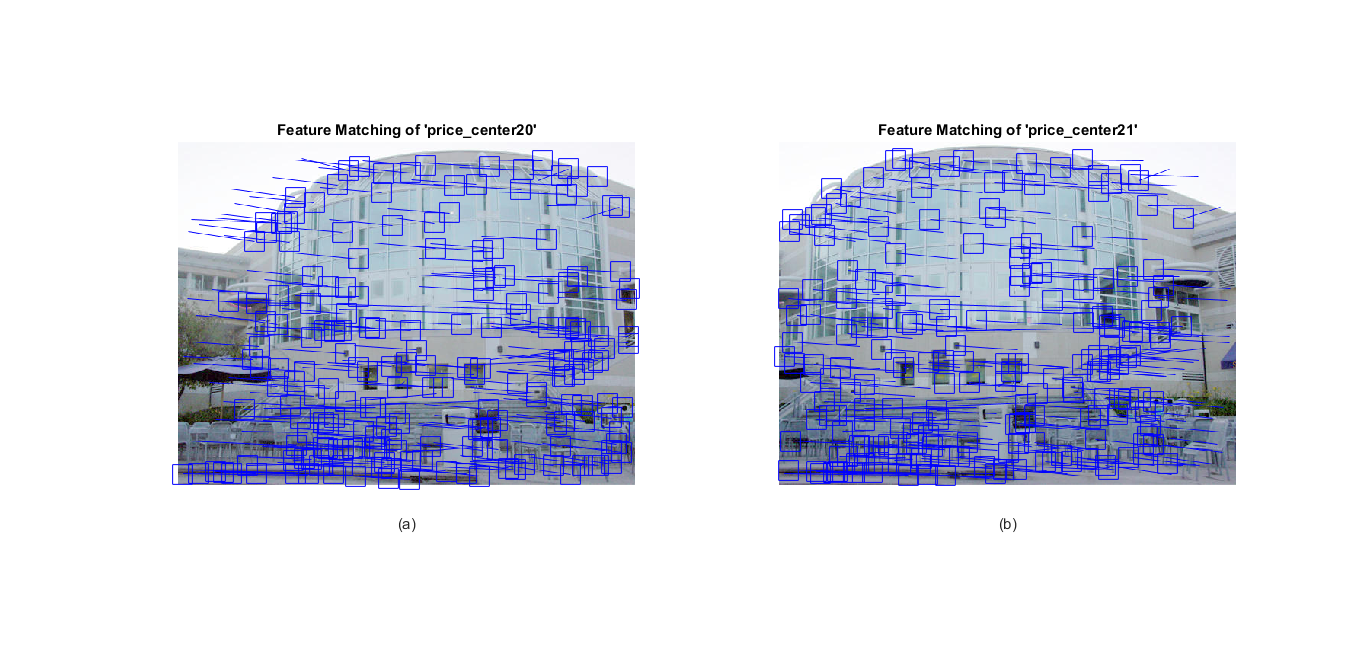
\includegraphics[width=6in]{FeatureMatch}
\caption{(a) shows matched features in \emph{price\_ center20.JPG}, (b) shows matched features in \emph{price\_ center21.JPG}.}
% \label{fig:images}
\end{figure} 

\end{enumerate}
\end{problemlist}

\begin{flushleft}
\large{\textbf{Appendix}}
\end{flushleft}

\lstinputlisting[language=Octave]{../src/main.m}
\lstinputlisting[language=Octave]{../src/CornerCoordinate.m}
\lstinputlisting[language=Octave]{../src/FeatureMatch.m}

\end{document}
